\documentclass[tikz,border=2pt]{standalone}
\usepackage{amsmath,amssymb}
\usepackage{tikz}
\usetikzlibrary{arrows.meta}

\begin{document}
% Three periods with demands (2,1,3) and the worked optimum: orders (2,2,2), stock carried
% x2 = 0, x3 = 1, x4 = 0, total cost 79.
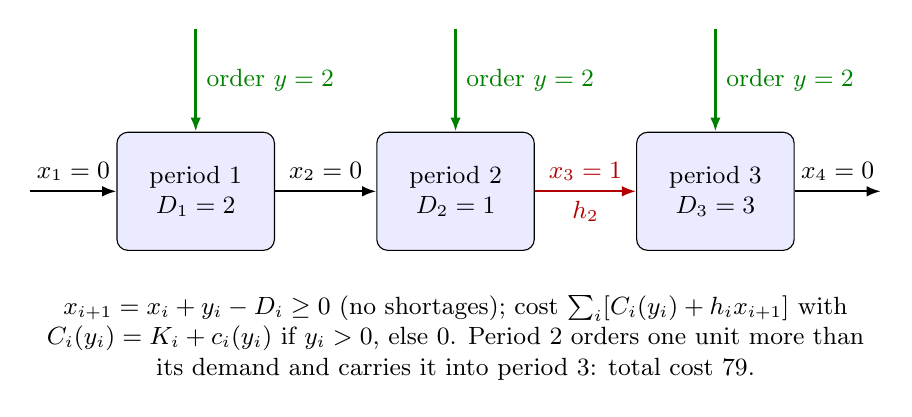
\begin{tikzpicture}[every node/.style={font=\small}, >={Latex[length=1.8mm]}, p/.style={draw, rounded corners=4pt, minimum width=2.0cm, minimum height=1.5cm, fill=blue!8, align=center}]
	\node[p] (p1) at (0,0) {period 1\\ $D_1=2$};
	\node[p] (p2) at (3.3,0) {period 2\\ $D_2=1$};
	\node[p] (p3) at (6.6,0) {period 3\\ $D_3=3$};
	\foreach \n/\y in {p1/2, p2/2, p3/2} {\draw[->, green!50!black, very thick] ([yshift=1.3cm]\n.north) -- (\n.north) node[midway, right] {order $y=\y$};}
	\draw[->, thick] (-2.1,0) -- (p1) node[midway, above] {$x_1=0$};
	\draw[->, thick] (p1) -- (p2) node[midway, above] {$x_2=0$};
	\draw[->, thick, red!70!black] (p2) -- (p3) node[midway, above] {$x_3=1$} node[midway, below] {$h_2$};
	\draw[->, thick] (p3) -- (8.7,0) node[midway, above] {$x_4=0$};
	\node[anchor=north, align=flush center, text width=10.4cm] at (3.3,-1.2) {$x_{i+1}=x_i+y_i-D_i\ge0$ (no shortages); cost $\sum_i[C_i(y_i)+h_ix_{i+1}]$ with $C_i(y_i)=K_i+c_i(y_i)$ if $y_i>0$, else $0$. Period 2 orders one unit more than its demand and carries it into period 3: total cost $79$.};
\end{tikzpicture}
\end{document}
